%% abtex2-modelo-trabalho-academico.tex, v-1.9.2 laurocesar
%% Copyright 2012-2014 by abnTeX2 group at http://abntex2.googlecode.com/ 
%%
%% This work may be distributed and/or modified under the
%% conditions of the LaTeX Project Public License, either version 1.3
%% of this license or (at your option) any later version.
%% The latest version of this license is in
%%   http://www.latex-project.org/lppl.txt
%% and version 1.3 or later is part of all distributions of LaTeX
%% version 2005/12/01 or later.
%%
%% This work has the LPPL maintenance status `maintained'.
%% 
%% The Current Maintainer of this work is the abnTeX2 team, led
%% by Lauro César Araujo. Further information are available on 
%% http://abntex2.googlecode.com/
%%
%% This work consists of the files abntex2-modelo-trabalho-academico.tex,
%% abntex2-modelo-include-comandos and abntex2-modelo-references.bib
%%

% ------------------------------------------------------------------------
% ------------------------------------------------------------------------
% abnTeX2: Modelo de Trabalho Academico (tese de doutorado, dissertacao de
% mestrado e trabalhos monograficos em geral) em conformidade com 
% ABNT NBR 14724:2011: Informacao e documentacao - Trabalhos academicos -
% Apresentacao
% ------------------------------------------------------------------------
% ------------------------------------------------------------------------

\documentclass[
	% -- opções da classe memoir --
	12pt,				% tamanho da fonte
	openright,			% capítulos começam em pág ímpar (insere página vazia caso preciso)
	twoside,			% para impressão em verso e anverso. Oposto a oneside
	a4paper,			% tamanho do papel. 
	% -- opções da classe abntex2 --
	%chapter=TITLE,		% títulos de capítulos convertidos em letras maiúsculas
	%section=TITLE,		% títulos de seções convertidos em letras maiúsculas
	%subsection=TITLE,	% títulos de subseções convertidos em letras maiúsculas
	%subsubsection=TITLE,% títulos de subsubseções convertidos em letras maiúsculas
	% -- opções do pacote babel --
	english,			% idioma adicional para hifenização
	french,				% idioma adicional para hifenização
	spanish,			% idioma adicional para hifenização
	brazil				% o último idioma é o principal do documento
	]{abntex2}

% ---
% Pacotes básicos 
% ---
\usepackage{lmodern}			% Usa a fonte Latin Modern			
\usepackage[T1]{fontenc}		% Selecao de codigos de fonte.
\usepackage[utf8]{inputenc}		% Codificacao do documento (conversão automática dos acentos)
\usepackage{lastpage}			% Usado pela Ficha catalográfica
\usepackage{indentfirst}		% Indenta o primeiro parágrafo de cada seção.
\usepackage{color}				% Controle das cores
\usepackage{graphicx}			% Inclusão de gráficos
\usepackage{microtype} 			% para melhorias de justificação
% ---
		
%%CUSTOM image paths
%Path relative to the main .tex file 
\graphicspath{ {./images/} }

% ---
% Pacotes adicionais, usados apenas no âmbito do Modelo Canônico do abnteX2
% ---
\usepackage{lipsum}				% para geração de dummy text
% ---

% ---
% Pacotes de citações
% ---
\usepackage[brazilian,hyperpageref]{backref}	 % Paginas com as citações na bibl
\usepackage[alf]{abntex2cite}	% Citações padrão ABNT

% --- 
% CONFIGURAÇÕES DE PACOTES
% --- 

% ---
% Configurações do pacote backref
% Usado sem a opção hyperpageref de backref
\renewcommand{\backrefpagesname}{Citado na(s) página(s):~}
% Texto padrão antes do número das páginas
\renewcommand{\backref}{}
% Define os textos da citação
\renewcommand*{\backrefalt}[4]{
	\ifcase #1 %
		Nenhuma citação no texto.%
	\or
		Citado na página #2.%
	\else
		Citado #1 vezes nas páginas #2.%
	\fi}%
% ---

% ---
% Informações de dados para CAPA e FOLHA DE ROSTO
% ---
\titulo{Enriquecimento de contexto com análise semântica para assistente virtual pessoal num cenário de Cidades Inteligentes}
\autor{Frederico Costa Galvão \\ Lucas Costa Sousa Milhomem}
\local{Goiânia, Brasil}
\data{2018}
\orientador{Marcelo Stehling de Castro}
\coorientador{Sandrerley Ramos Pires}
\instituicao{%
UNIVERSIDADE FEDERAL DE GOIÁS \par
ESCOLA DE ENGENHARIA ELÉTRICA, MECÂNICA E DE COMPUTAÇÃO
  \par}
 \tipotrabalho{Monografia de Graduação}
% O preambulo deve conter o tipo do trabalho, o objetivo, 
% o nome da instituição e a área de concentração 
\preambulo{Monografia apresentada como requisito parcial para a obtenção do título de Bacharel em Engenharia no curso de graduação em Engenharia de Computação da Escola de Engenharia Elétrica, Mecânica e de Computação da Universidade Federal de Goiás.}
% ---

% ---
% Configurações de aparência do PDF final

% alterando o aspecto da cor azul
\definecolor{blue}{RGB}{41,5,195}

% informações do PDF
\makeatletter
\hypersetup{
     	%pagebackref=true,
		pdftitle={\@title}, 
		pdfauthor={\@author},
    	pdfsubject={\imprimirpreambulo},
	    pdfcreator={LaTeX with abnTeX2},
		pdfkeywords={abnt}{latex}{abntex}{abntex2}{trabalho acadêmico}, 
		colorlinks=true,       		% false: boxed links; true: colored links
    	linkcolor=blue,          	% color of internal links
    	citecolor=blue,        		% color of links to bibliography
    	filecolor=magenta,      		% color of file links
		urlcolor=blue,
		bookmarksdepth=4
}
\makeatother
% --- 

% --- 
% Espaçamentos entre linhas e parágrafos 
% --- 

% O tamanho do parágrafo é dado por:
\setlength{\parindent}{1.3cm}

% Controle do espaçamento entre um parágrafo e outro:
\setlength{\parskip}{0.2cm}  % tente também \onelineskip

% ---
% compila o indice
% ---
\makeindex
% ---

% ----
% Início do documento
% ----
\begin{document}

% Retira espaço extra obsoleto entre as frases.
\frenchspacing 

% ----------------------------------------------------------
% ELEMENTOS PRÉ-TEXTUAIS
% ----------------------------------------------------------
% \pretextual

% ---
% Capa
% ---
\imprimircapa
% ---

% ---
% Folha de rosto
% (o * indica que haverá a ficha bibliográfica)
% ---
\imprimirfolhaderosto*
% ---

% ---
% Inserir a ficha bibliografica
% ---

% Isto é um exemplo de Ficha Catalográfica, ou ``Dados internacionais de
% catalogação-na-publicação''. Você pode utilizar este modelo como referência. 
% Porém, provavelmente a biblioteca da sua universidade lhe fornecerá um PDF
% com a ficha catalográfica definitiva após a defesa do trabalho. Quando estiver
% com o documento, salve-o como PDF no diretório do seu projeto e substitua todo
% o conteúdo de implementação deste arquivo pelo comando abaixo:
%
% \begin{fichacatalografica}
%     \includepdf{fig_ficha_catalografica.pdf}
% \end{fichacatalografica}

\begin{fichacatalografica}
	\sffamily
%	\vspace*{\fill}					% Posição vertical
	\begin{center}					% Minipage Centralizado
	\fbox{\begin{minipage}[c][8cm]{13.5cm}		% Largura
	\small
	\imprimirautor / \imprimirtitulo \par
	%Sobrenome, Nome do autor
	
	\imprimirtipotrabalho~--~\imprimirinstituicao,\imprimirlocal,\imprimirdata
	\newline
	\vspace{0.5cm}
	\hspace{0.5cm} \thelastpage p. : il. (algumas color.) ; 30 cm.
	\newline
    \hspace{0.5cm} \imprimirorientadorRotulo~\imprimirorientador
	\newline
		1. Web semântica \par
		2. Cidades inteligentes \par
		3. Processamento de linguagens naturais \par
		I. {\imprimirinstituicao}
		II. \imprimirtitulo
	\end{minipage}}
	\end{center}
	\newpage
\end{fichacatalografica}
% ---

% ---
% Inserir folha de aprovação
% ---

% Isto é um exemplo de Folha de aprovação, elemento obrigatório da NBR
% 14724/2011 (seção 4.2.1.3). Você pode utilizar este modelo até a aprovação
% do trabalho. Após isso, substitua todo o conteúdo deste arquivo por uma
% imagem da página assinada pela banca com o comando abaixo:
%
% \includepdf{folhadeaprovacao_final.pdf}
%
\begin{folhadeaprovacao}
  \begin{center}
    {\ABNTEXchapterfont\large\imprimirautor}

    \vspace*{\fill}\vspace*{\fill}
    \begin{center}
%    {\par \Large  \textbf{\imprimirinstituicao} \par \par}
    {\par \Large  \textbf{FOLHA DE APROVAÇÃO} \\ \par}
      \ABNTEXchapterfont\bfseries\Large\imprimirtitulo
    \end{center}
    \vspace*{\fill}
    
    \hspace{.45\textwidth}
    \begin{minipage}{.5\textwidth}
        \imprimirpreambulo
    \end{minipage}
    \vspace*{\fill}
   \end{center}
        
   Monografia defendida e aprovada em \imprimirlocal,  14 de dezembro de 2018, pela banca examinadora constituída por:

   \assinatura{\textbf{\imprimirorientador} \\ Orientador} 
   \assinatura{\textbf{Sandrerley Ramos Pires } \\ Coorientador}
   \assinatura{\textbf{Gustavo Dias de Oliveira} \\  Engenheiro convidado}
   %\assinatura{\textbf{Professor} \\ Convidado 3}
   %\assinatura{\textbf{Professor} \\ Convidado 4}
      
   \begin{center}
    \vspace*{0.5cm}
    {\large\imprimirlocal}
    \par
    {\large\imprimirdata}
    \vspace*{1cm}
  \end{center}
  
\end{folhadeaprovacao}
% ---

%%%TODO revisar dedicatória com o Lucas
% ---
% Dedicatória
% ---
\begin{dedicatoria}
   \vspace*{\fill}
   \centering
   \noindent
   \textit{ Este trabalho é dedicado aos professores do curso de Engenharia de Computação que souberam manter sempre ativos em nós o interesse e a curiosidade do aprendizado constante, e aos futuros pesquisadores e profissionais que terão o papel crucial de construir e manter uma internet mais inteligente que a atual. } \vspace*{\fill}
\end{dedicatoria}
% ---

%%%TODO redigir agradecimentos com o Lucas
% ---
% Agradecimentos
% ---
\begin{agradecimentos}
Os agradecimentos principais são direcionados aos professores  {\imprimirorientador} e Sandrerley Ramos Pires.

\end{agradecimentos}
% ---

% ---
% Epígrafe
% ---
\begin{epigrafe}
    \vspace*{\fill}
	\begin{flushright}
		\textit{``A verdade raramente é pura, e nunca é simples. \\
		(Oscar Wilde - The Importance of Being Earnest)}
	\end{flushright}
\end{epigrafe}
% ---

% ---
% RESUMOS
% ---

% resumo em português
\setlength{\absparsep}{18pt} % ajusta o espaçamento dos parágrafos do resumo
\begin{resumo}
 Nos últimos anos o consumo de conteúdo virtual aumentou significativamente, entretanto este ainda não está estruturado de maneira preparada para a dimensão prevista pelos projetos de cidades inteligentes em planejamento. A reorganização da internet pelos conceitos da semântica que levará a web ao patamar de Web 3.0 (Web Semântica) está sendo colocada em prática pela Internet das Coisas e por abordagens modernas de processamento de dados, porém a tecnologia necessária para atender as demandas estipuladas ainda se encontra desafiada. Propõe-se, portanto, pesquisa e desenvolvimento de um sistema de mapeamento e gerência de informações pessoais baseado em análise semântica de conteúdo já consumido via extensões de browsers e aplicativos móveis com o objetivo de desenvolver um assistente virtual pessoal de memória e de consumo de conteúdo.

 \textbf{Palavras-chaves}: web 3. web semântica. cidades inteligentes. internet das coisas. gerência de informação pessoal. processamento de linguagens naturais.
\end{resumo}

% resumo em inglês
\begin{resumo}[Abstract]
 \begin{otherlanguage*}{english}
   In the latest years, virtual content consumption increased significantly, but that content still isn't well structured enough to handle the order of magnitude predicted by the ongoing smart city projects. The reorganization of the internet through semantic means that will take it to the level of Web 3.0 (Semantic Web) is being put into practice by the Internet of Things and by modern data processing approaches. Nevertheless, the technology needed to satisfy the demands stipulated is still being challenged. We propose, then, research and development of a system to map and manage personal information based on semantic analysis of consumed content through browser extensions and mobile applications with the intent to develop a virtual personal assistant on memory and content consumption.

   \vspace{\onelineskip}
 
   \noindent 
   \textbf{Key-words}: web 3. semantic web. smart city. internet of things. personal information management. natural language processing.
 \end{otherlanguage*}
\end{resumo}
% ---

% ---
% inserir lista de ilustrações
% ---
\pdfbookmark[0]{\listfigurename}{lof}
\listoffigures*
\cleardoublepage
% ---

% ---
% inserir lista de tabelas
% ---
\pdfbookmark[0]{\listtablename}{lot}
\listoftables*
\cleardoublepage
% ---

% ---
% inserir lista de abreviaturas e siglas
% ---
\begin{siglas}
  \item[IoT] Internet of Things
  \item[GDPR] General Data Protection Regulation
\end{siglas}
% ---

% ---
% inserir o sumario
% ---
\pdfbookmark[0]{\contentsname}{toc}
\tableofcontents*
\cleardoublepage
% ---



% ----------------------------------------------------------
% ELEMENTOS TEXTUAIS
% ----------------------------------------------------------
\textual

% ----------------------------------------------------------
% PARTE
% ----------------------------------------------------------
\part{Introdução}
% ----------------------------------------------------------

\chapter{Contexto do problema} \label{c:contexto_do_problema}

A seguir, serão abordados conceitos utilizados ao longo do trabalho, que envolvem o processamento natural de linguagens, cidades inteligentes, assistentes virtuais pessoais e a  privacidade na Era da Internet das Coisas.

\section{Processamento natural de linguagens} \label{s:processamento_natural_de_linguagens}

Processamento de Linguagem Natural (PLN) consiste no desenvolvimento de modelos computacionais para a realização de tarefas que dependem de informações expressas em alguma língua natural, a pesquisa em PLN está voltada, essencialmente, a três aspectos da comunicação em língua natural:
\begin{itemize}
\item  Som: fonologia
\item  Estrutura: morfologia e sintaxe
\item  Significado: semântica e pragmática
\end{itemize}
A \textbf{fonologia} está relacionada ao reconhecimento dos sons que compõem as palavras de uma língua. A \textbf{morfologia} reconhece as palavras em termos das unidades primitivas que a compõem. A \textbf{sintaxe} define a estrutura de uma frase, com base na forma como as palavras se relacionam nessa frase.  A \textbf{semântica} associa significado a uma estrutura sintática, em termos dos significados das palavras que a compõem. A \textbf{pragmática} verifica se o significado associado à uma estrutura sintática é realmente o significado mais apropriado no contexto considerado.

Com uma grande quantidade de páginas, a web se constitui hoje quase todas usando linguagem natural, com isso um agente que deseja adquirir conhecimento tem que entender a ambiguidade e confusão da linguagem humana (RUSSELL; NORVIG, 2013).

As linguagens naturais não podem ser descritas como um conjunto de sentenças definidas. Com isso se torna melhor definir um modelo de linguagem natural usando probabilidade sobre sentenças em vez de um conjunto definido(RUSSELL; NORVIG, 2013).

Linguagens naturais são ambíguas, pode-se tomar de exemplo o “Ele viu o banco”, onde pode significar que ele viu uma peça de mobília ou uma instituição financeira. Com isso não se pode falar de um significado e sim de uma probabilidade sobre o significado(RUSSELL; NORVIG, 2013).

O Processamento de Linguagem Natural (PLN) tal como construído por (JUNIOR, 2008), tem duas abordagens principais, que são a baseada em texto e a baseada em diálogo. A abordagem baseada em texto tem como principal foco na busca de documentos e resumo e compreensão de textos(JUNIOR, 2008).A abordagem baseada em diálogo tem crescimento com a interface entre máquinas e humanos(JUNIOR, 2008). 

O Processamento de Linguagem Natural tem como principal a etapa de pré-processamento, onde serão definidas e reconhecidas às sentenças e classificação das palavras a sua função sintática(JUNIOR, 2008).

\section{Cidades inteligentes} \label{s:cidades_inteligentes}

Por volta de 475 a.C., na Grécia, foi definido o primeiro modelo de urbanização propriamente dito, no qual a cidade passou a ser regularmente dividida. Tal formato foi difundido por Hippodamus de Mileto, filósofo e arquiteto considerado por muitos historiadores como o pai do planejamento urbano.

Nessa época, a cidade apresentava um traçado ortogonal, denominado plano hipodâmico (ABIKO \textit{et al.}, 1995). Entre suas teorias, Hippodamus pregava que, em cidades com mais de 10 mil habitantes, deveria haver uma divisão entre classes (artesã, agrícola e guerreira) e o território teria partes com funções definidas. Uma delas seria reservada a propriedades particulares, outra teria domínio público e a terceira seria consagrada aos deuses.

Assim, dentro dessas zonas haveria setores residenciais, o porto comercial e o militar, a ágora (local que caracterizava o centro das atividades da polis grega) e os santuários (ABIKO \textit{et al.}, 1995).
Outro modelo de cidade a ser considerado no histórico da urbanização é o romano. Seu traçado teve origem nos acampamentos militares (GOITIA, 1992 \textit{apud} ABIKO \textit{et al.}, 1995), dando à cidade romana uma forte característica relacionada à defesa, reforçada muitas vezes por muros que circundavam seu território.

Além disso, um fator inserido neste modelo foi o da convivência civil, na forma de uma praça especial que concentrava os equipamentos públicos e o lazer da época, como circos, anfiteatros e termas (HAROUEL, 1990 \textit{apud} ABIKO \textit{et al.}, 1995).

Posteriormente, na Idade Média, as cidades passam a funcionar sob uma nova ordem: o sistema feudal. Nele, tomou força uma sociedade estamental, baseada na obrigação servil e com a presença integral da religião na sociedade, sob a atuação do clero (ARRUDA, 1993 \textit{apud} ABIKO \textit{et al.}, 1995).

A cidade medieval era fortificada e localizada em locais de difícil acesso, provocando o isolamento dos feudos. Devido a
isso, seu traçado muitas vezes era espontâneo e condicionado pela irregularidade da topografia local, embora o padrão radiocêntrico de ruas secundárias fosse um dos mais comuns (GOITIA, 1992 \textit{apud} ABIKO \textit{et al.}, 1995).

No século XV, com o Renascimento, o urbanismo se direciona à organização geométrica ideal do território, com predominância da regularidade, simetria e de proporções rígidas entre as vias e praças (ABIKO \textit{et al.}, 1995).

Na ocasião, a paisagem urbana adquiriu um formato de tabuleiro e foi fruto do exercício intelectual (GOITIA, 1992 \textit{apud} ABIKO \textit{et al.}, 1995) para ocupação dos grandes espaços vazios com a realização de programas de colonização e urbanização (BENEVOLO, 1993 \textit{apud} ABIKO \textit{et al}., 1995).

Por outro lado, há o surgimento das grandes cidades e as capitais políticas ganham importância diferenciada, concentrando os instrumentos políticos do Estado nacional e extinguindo a cidade soberana (ABIKO \textit{et al.}, 1995).

No século XIX, com a Revolução Industrial, houve um grande incremento populacional. A cidade industrial foi desenvolvida principalmente com a ampliação de bairros ocupados por operários e a ausência de um sistema capaz de controlar de forma eficaz o crescimento urbano. Assim, a cidade tornou-se cada vez mais compactada devido à construção de novos edifícios e o adensamento populacional se intensificou, tornando o congestionamento e a insalubridade fatores marcantes da época (ABIKO \textit{et al.}, 1995).

\section{Assistentes virtuais pessoais} \label{s:assistentes_virtuais_pessoais}

Podemos chamar de Assistente Virtual os agentes de interface que são representados através de personagens que tem como foco melhorar a interação entre humanos e computadores.

Estes personagens são normalmente associados a algum tipo de mecanismo de inteligência artificial que lhes permitem detectar estímulos externos e responder a estes adequadamente. Trata-se do emprego de uma metáfora em que um assistente pessoal colabora com o usuário no mesmo ambiente de trabalho (Maes, 1994).

Muitas pesquisas têm investigado o impacto dos assistentes virtuais no desenvolvimento da aprendizagem interativa 1 . Shaw e Johnson (1999) descrevem experimentos com um professor virtual que orienta alunos em atividades interativas online. Craig \textit{et al.} (2002) investigam diferentes efeitos no processo de aprendizagem de alunos submetidos a personagens estáticos e animados.

Sims (2000) apresenta resultados sobre o uso de personagens virtuais no ensino da língua de sinais para crianças com deficiência auditiva. Outros estudos também mostram que a presença da figura humana tem um efeito positivo em experiências interativas com estudantes.

Andre \textit{et al.} (1999) identificaram que estudantes consideram o objeto de estudo menos difícil quando existe a presença de um assistente virtual. O mesmo estudo mostrou que os estudantes prestam mais atenção aos importantes detalhes da página, em função da presença do assistente.

\section{Privacidade na Internet das Coisas} \label{s:privacidade_na_internet_das_coisas}

Temos cerca de dois bilhões de usuários conectados à Internet, se comunicando, navegando na Web, acessando os mais diversos tipos de conteúdo multimídia, jogos, redes sociais e outras aplicações.

Com o crescente incremento das infra-estruturas de redes e popularização em massa da internet de alta velocidade, emerge um avanço relacionado à utilização da internet tornando-a uma plataforma global para deixar máquinas e objetos inteligentes capazes de comunicarem-se de forma autônoma (MIORANDI \textit{et al.}, 2012).

Gao e Bai (2014) destacam que durante a próxima década, a rede inter-existirá como um tecido sem costura de redes clássicas e objetos ligados em rede. O conteúdo e serviços estarão em torno das pessoas, sempre disponível, facilitando a comunicação e abrindo o caminho para novas aplicações, possibilitando novas formas de trabalho, de interação, de entretenimento, fazendo com que um novo padrão de vida seja desenvolvido.

Este novo padrão de vida, torna-se possível através dos avanços das TICs até uma nova concepção definida como Internet of Things - IoT. O termo Internet of Things foi cunhado pela primeira vez em 1999 por Ashton, um dos pioneiros da tecnologia britânica que ajudou a desenvolver o conceito (GUBBI \textit{et al.}, 2013).

A IoT visa estender os benefícios da internet proporcionando uma conectividade constante, desenvolvendo uma capacidade de controle remoto e compartilhamento de dados para os bens no mundo físico (PEOPLES \textit{et al.}, 2013).

A Internet das Coisas - IoT advém do conceito de presença generalizada em torno das pessoas e de uma variedade de coisas ou objetos, através de Radio Frequency IDentification - RFID, sensores, atuadores, gadget como smartphones, tablet, televisores, pulseiras e relógios inteligentes, \textit{etc.}, por meio de esquemas de endereçamento exclusivos que são capazes de interagir uns com os outros e cooperar com os seus vizinhos para alcançar objetivos comuns (ATZORI; IERA; MORABITO, 2010).

Dentro dessa perspectiva, o termo Internet of Things - IoT é amplamente usado para se referir a ambos: a rede global resultante da interligação dos objetos inteligentes; ao conjunto de tecnologias de apoio necessárias para concretizar essa visão; e o conjunto de aplicações e serviços que alavancam tais tecnologias para abrir novas oportunidades de negócios e de mercados (MIORANDI \textit{et al.}, 2012).

A eficácia da IoT reside no alto impacto que ela se dispõe a proporcionar sobre diversos aspectos do cotidiano de vida e comportamento de usuários potenciais (PEOPLES \textit{et al.}, 2013).

Do ponto de vista de um usuário privado, os efeitos mais evidentes da introdução da IoT estão em suas funções assistidas, como em cuidados com a saúde, orientação de aprendizagem e controle doméstico, são apenas alguns exemplos dos campos de aplicação da IoT.

Da mesma forma, a partir da perspectiva dos usuários de negócios, as consequências mais aparentes serão igualmente visíveis em áreas como automação e manufatura industrial, logística, processo de gestão e tomada de decisão, transporte inteligente de pessoas e bens (ATZORI; IERA; MORABITO, 2010).

Com uma variada coleta de dados e informações, para variados fins, no cotidiano das pessoas, seja em ambientes domésticos de usuários privados ou em ambientes profissionais de usuários de negócios, a coleta autônoma dos dados e das informações das pessoas torna a privacidade uma das principais preocupações éticas com relação à Internet das Coisas.

Entendida por Chabridon \textit{et al.} (2014) como uma questão crucial que pode limitar a implantação da visão IoT seja para usuários privados ou para organizações. Chabrindon et al. (2014) e Weber e Weber (2010) ressaltam que a privacidade é fundamental para o controle deste novo ambiente complexo.

A troca de dados invisível e constante entre as coisas e as pessoas, e entre as coisas e outras coisas, irá ocorrer de forma que os proprietários e criadores desses dados não sejam identificados.

A própria escala e capacidade das novas tecnologias vai ampliar este problema. O termo privacidade transmite um grande número de conceitos e ideias. Comumente associa-se privacidade com a noção de um indivíduo que controla o acesso a sua informação pessoal.

Weber e Weber (2010) identificam três áreas relacionadas com a privacidade, sendo elas: o espaço físico, que pode ser compreendido como um escudo contra objetos indesejados ou sinais, neste sentido a privacidade está perto de segurança de infra-estrutura; o poder de tomada de decisão em relação ao fluxo de informações com o objetivo de proteger a liberdade de uma pessoa a fazer escolhas a respeito de seus dados; e o controle de um indivíduo sobre o processamento da informação compreendendo a aquisição, divulgação e uso de informações pessoais.

No entanto, Chabrindon \textit{et al.} (2014) afirmam que preservar a privacidade através do isolamento não é mais uma opção no mundo da informação e da comunicação de hoje. Para um contexto de ambiente inteligente gerado pela Internet das Coisas, onde as aplicações tornassem de fácil usabilidade e as informações são disponibilizadas de maneira muitas vezes imperceptíveis, a privacidade é geralmente percebida pelos usuários como uma expectativa de estar em um estado de proteção sem ter que persegui-lo ativamente.

Nessa linha, Marx e Murky (2001) identificaram quatro níveis de privacidade perceptíveis pelas pessoas, estes níveis são posteriormente destacados por Chabrindon \textit{et al.} (2014) para definir a maneira como as pessoas percebem as violações a sua privacidade, sendo estes níveis nomeados como fronteiras: a \textbf{fronteira natural} impede a sua presença (ou sentimentos ou emoção) de ser percebido através de um dos sentidos humanos, como paredes, portas, cartas seladas, telefone e email representam fronteiras naturais para observação; a \textbf{fronteira da sociedade} envolve expectativas das pessoas para certos papéis sociais (médicos, membros do clero, advogados) profissionais que não vão divulgar informações confidenciais; a \textbf{fronteira espacial ou temporal} que separa a informação dos vários períodos ou aspectos da vida da pessoa; e a \textbf{fronteira dos efeitos efêmeros ou transitórios}, tais fronteiras baseiam-se na ideia de que a interação e comunicação são esquecidas em breve.

Nota-se que a IoT, enquanto inovação tecnológica que envolve questões de privacidade de dados e informações de usuários, ganha espaço nas discussões acaloradas em meios acadêmicos e profissionais.

Assim, com vistas a contribuir para amplificação das discussões este texto visa discutir, de modo conceitual, os mais relevantes elementos que compõem o fenômeno da IoT. Para isso, o escrito divide-se em cinco sessões: esta introdução como primeira etapa; três sessões teóricas que versam sobre a origem da internet das coisas; privacidade e a IoT; e perspectivas legais da privacidade da informação. E, por fim, são feitas as considerações finais na tentativa de fomentar novas propostas de estudo.	

\chapter{Introdução à solução proposta} \label{c:introducao_a_solucao_proposta}

A proposta do trabalho é explorar a implementação de um sistema de coleta, processamento, enriquecimento, e aplicação de dados em serviços de assistência virtual de memória e de consumo de conteúdo ao usuário.

As ferramentas utilizadas e descritas neste focam na plataforma Java/JVM, por questões de familiaridade, acessibilidade, eficiência e comunidade, visto que a linguagem de programação Java ainda possui imensa relevância no mundo acadêmico e no mercado.

Este capítulo introduz cada uma das etapas de maneira superficial com o objetivo de delinear o fluxo completo do sistema proposto sem se apegar aos detalhes de implementação.

A modelagem de um sistema computacional eficiente de coleta, processamento, enriquecimento e aplicação de dados pode se beneficiar de modelos já comprovados por estudos de neurociência, processos cognitivos, e psicologia experimental de processos mnemônicos.

A lei da contiguidade temporal e espacial reforça a relevância destes modelos, e a eficiência em inferência de relacionamentos entre diversos eventos atingida por eles é copiosamente comprovada pela literatura \cite{Polyn2011SemanticCA}.

\section{Coleta de dados} \label{s:coleta_de_dados}

Entende-se que a riqueza do sistema está na diversidade e quantidade de dados coletados. Considerando que os modelos de cidades inteligentes emergentes possibilitam a coleta de inúmeros fluxos de dados diferentes por dispositivos pessoais e compartilhados, fica claro que tal sistema alcançaria um nível de complexidade e alcance contextual que nenhuma outra estrutura pode oferecer. 

\section{Processamento de dados} \label{s:processamento_de_dados}

O sistema prevê que várias camadas de tratamento e processamento de dados serão necessárias para que uma cidade inteligente consiga fornecer de maneira escalável e relevante uma interface de consumo de dados às camadas posteriores do sistema.

Algoritmos de normalização e extração de dados farão com que informação irrelevante ou desnecessária seja removida ou ofuscada a fim de discernir informação de contexto.

O uso de diversas abordagens de processamento de linguagens naturais é obrigatório, visto que alguns dos canais de coleta de dados se tratam de dados textuais que quase sempre envolvem alguma entidade ou domínio que possa ser transformado em metadado temporal ou georreferenciado.

\section{Enriquecimento de contexto} \label{s:enriquecimento_de_contexto}

Apesar das outras etapas serem de extrema importância, é papel do enriquecimento de contexto agregar valor à informação e conhecimento disponibilizados à aplicação de assistente virtual além do que as ferramentas clássicas e especializadas conseguem fornecer hoje.

A identificação de relacionamentos temporais, georreferenciais, ou de entidades é o papel mais importante de toda a pilha, e um resultado satisfatório nesta etapa depende de múltiplos sistemas de bancos de dados especialistas em sintonia com a aplicação de consumo desses dados.

É importante ressaltar que a eficácia do processo de enriquecimento de contexto de múltiplas fontes de dados tem dependência relevante da qualidade do processamento e tratamento de dados feito na etapa anterior.

\section{Aplicação dos dados} \label{s:aplicacao_dos_dados}

Uma vez que uma camada de distribuição de dados e metadados, ambos bem tratados e processados, seja criada e implementada de forma escalável e bem definida sob as premissas de um modelo completo de governança algorítmica de cidades inteligentes, inúmeras aplicações podem ser implementadas com o apoio de empresas parceiras a fim de fornecer serviços ao usuário final e aumentar de forma generalizada e acessível a qualidade de vida dos habitantes da cidade em questão.

Este trabalho se limita em planejar e discorrer sobre a implementação de sistemas que não dependam de um modelo de cidade inteligente ativo, para que resultados possam ser atingidos e demonstrados independente da sua implantação.

% ----------------------------------------------------------
% PARTE
% ----------------------------------------------------------
\part{Desenvolvimento}
% ----------------------------------------------------------

\chapter{Coleta de dados} \label{c:coleta_de_dados}

Inúmeras fontes de dados podem ser consideradas num modelo completo de cidade inteligente e no contexto de um cidadão moderno, que faz uso de todos os dispositivos de integração e automação disponíveis.

Essas fontes geralmente produzem conjuntos de dados caracterizados em principalmente duas dimensões: área de impacto e contexto de origem. A área de impacto de um conjunto de dado diz respeito aos elementos influenciadores e influenciados por tais dados, enquanto o contexto de origem caracteriza os elementos geradores dos dados de acordo com seu universo de origem.

\section{Individual \textit{versus} Social} \label{s:individual_vs_social}

Dispositivos privados ou residenciais quase sempre estarão focando os processos de coleta no usuário proprietário do elemento coletor, que é também dono de toda ou boa parte da informação.

Esses dados são classificados como \textit{individuais} e serão, portanto, quase sempre utilizados a fim de fornecer serviços e qualidade de vida pro contexto deste usuário. Isso engloba algumas premissas de privacidade e de propriedade de dados de projetos de cidades inteligentes e de regulação como o GDPR \cite{eu:gdpr} na Europa.

A manutenção e aplicação de dados individuais ocorrerá, na grande maioria dos casos, sob demanda e acordo do próprio usuário, que tem o poder de intervir e interromper, direta e imediatamente, os processos envolvendo tais dados.

Já os meios de coleta de dados coletivos, geralmente ligados a ambientes compartilhados ou à própria infraestrutura da cidade, são responsáveis pela coleta de dados \textit{sociais} que envolvem o coletivo, tendo às vezes um grupo de indivíduos como fonte de dados anonimizada ao invés de individualmente identificados.

Estudos anteriores de engenharia social serão aplicados nessa categoria de dados com mais frequência, pois o comportamento coletivo tem o potencial de, ao mesmo tempo, gerar dados extremamente valiosos e impactar o meio social de maneira negativa.

Entende-se que tanto os modelos de cidades inteligentes quanto as configurações de uso de um sistema como esse precisam levar em consideração atributos humanos no processo de representação social no modelo \cite{huso17}.

\section{Mundo digital \textit{versus} analógico} \label{s:mundo_digital_vs_analogico}

Apesar de toda e qualquer informação que trafega em um sistema assistente virtual e em uma cidade inteligente, ser obrigatoriamente digitalizada em algum momento antes de entrar nas etapas de processamento e armazenamento de dados, a origem desses dados pode diferir significativamente.

Informações que possuem origem já no mundo digital, como as geradas por interações homem-máquina, são mais facilmente abstraídas e representadas do que as que possuem origem analógica, como as geradas por interações homem-cidade.

\section{Fontes de dados consideradas} \label{s:fontes_de_dados_consideradas}

Nesta seção serão descritas algumas fontes de dados presentes em um contexto urbano inserido no contexto maior de uma cidade inteligente, com a classificação de área de impacto e contexto de origem de seus dados, assim como exemplos concretos de eventos e informações delas extraídas.

Se os últimos anos provaram algo sobre a gama de possibilidades de coleta de dados em projetos de cidades inteligentes, é que a lista de fontes de dados cruciais para o bom funcionamento de um sistema deste porte está em constante e íngreme crescimento \cite{lavaprotocols:smartcity}.

É importante ressaltar, no entanto, que várias fontes de dados transitam entre o mundo digital e analógico e entre impacto individual e social com facilidade, já que alguns desses canais são ambivalentes e podem ser aplicados, em diferentes circunstâncias, para fins diversos ao mesmo tempo. Portanto, a classificação nessas duas dimensões dos exemplos que seguem são apenas um indicador de predominância, não de exclusividade.

%%------
\subsection{Navegador (\textit{browser})}

\textbf{Área de impacto}: Individual; \textbf{Contexto de origem}: Digital;

\textbf{Descrição}: Tudo que possa ser acessado diretamente pelo browser, que tenha uma URL e que tenha conteúdo HTML extraível;

\textbf{Exemplos}: artigos lidos no Medium, vídeos assistidos no Youtube, filmes e séries assistidos na Netflix, músicas ouvidas no Spotify, páginas visitadas no Facebook.

%%------
\subsection{Sistema operacional \textit{desktop}}

\textbf{Área de impacto}: Individual; \textbf{Contexto de origem}: Digital;

\textbf{Descrição}: Tudo que possa ser extraído de atividade do usuário com \textit{timestamp} a nível de sistema operacional (Linux, Windows, macOS) que não tenha vindo de uma URL pelo \textit{browser};

\textbf{Exemplos}: arquivos abertos, programas executados, qualquer outro evento que indique atividade.

%%------
\subsection{Sistema operacional móvel}

\textbf{Área de impacto}: Individual; \textbf{Contexto de origem}: Digital;

\textbf{Descrição}: Tudo que possa ser extraído de atividade do usuário no mundo mobile (\textit{smartphones, smartwatches});

\textbf{Exemplos}: aplicativos abertos, conectividade, GPS.

%%------
\subsection{Web 3.0 - \textit{Personal Online Data store} (PODs)}

\textbf{Área de impacto}: Individual; \textbf{Contexto de origem}: Digital;

\textbf{Descrição}: Tudo que possa ser consumido e extraído de \textit{PODs} ou de bancos de dados individuais semelhantes. A definição de \textit{PODs} usada aqui é a mesma do projeto \textit{Solid} da Web 3.0\footnote{\url{https://solid.inrupt.com/how-it-works}}.

%%------
\subsection{\textit{Global Positioning System} (GPS)}

\textbf{Área de impacto}: Individual; \textbf{Contexto de origem}: Analógico;

\textbf{Descrição}: Pode vir de um smartphone com alta precisão, pode vir de um desktop ou notebook com baixa precisão, pode vir de um GPS automotivo, etc;

%%------
\subsection{\textit{Biofeedback}}

\textbf{Área de impacto}: Individual; \textbf{Contexto de origem}: Analógico;

\textbf{Descrição}: Pode vir de dispositivos intracutâneos ou de acessórios médicos externos;

\textbf{Exemplos}: controle de ansiedade, monitoramento e alívio de asma e dos efeitos colaterais da quimioterapia.

%%------
\subsection{Redes sociais e mensageiros}

\textbf{Área de impacto}: Social; \textbf{Contexto de origem}: Digital;

\textbf{Descrição}: Relacionamentos do usuário com outros usuários e outras entidades como empresas ou comunidades;

%%------
\subsection{Sistemas políticos e administrativos}

\textbf{Área de impacto}: Social; \textbf{Contexto de origem}: Digital;

\textbf{Descrição}: Pode vir de sistemas proprietários de gestão de recursos, ou de sistemas abertos de gerenciamento de diversos departamentos que compõem a parte administrativa de uma cidade ou estado;

\textbf{Exemplos}: controle de despesas municipais, abertura ou resultado de votações, licitações e processos de reforma de infraestrutura.

%%------
\subsection{Mobilidade inteligente}

\textbf{Área de impacto}: Social; \textbf{Contexto de origem}: Analógico;

\textbf{Descrição}: Toda informação que um sistema de mobilidade conectada possa fornecer a outros sistemas ou para os cidadãos;

\textbf{Exemplos}: previsão de chegada e planejamento de rota de transporte público, controle inteligente de estacionamento, carga de bateria de carros elétricos.

%%------
\subsection{Proximidade via GPS}

\textbf{Área de impacto}: Social; \textbf{Contexto de origem}: Analógico;

\textbf{Descrição}: Tudo que possa ser relacionado entre entidades diferentes (usuários, empresas, estabelecimentos, eventos) considerando a distância geográfica entre elas.
\chapter{Processamento de dados}

Esta etapa tem como responsabilidade consumir a interface exposta pela coleta de dados brutos e expôr à camada seguinte, de enriquecimento de contexto, uma interface de consumo de dados úteis e bem formatados. Diferentes tipos de dados demandam diferentes abordagens e técnicas de processamento textual ou de extração de metadados. Também por isso, a etapa de processamento de dados será responsável por uma das camadas de armazenamento de dados mais importante, e a multidisciplinaridade das tecnologias utilizadas é fundamental para atingir eficiência e escalabilidade em todas as áreas de atuação.

\section{Dado útil vs dado bruto}

Alguns dos canais de coleta de dados extraem informação bruta de um contexto às vezes muito mais rico e diversificado do que o necessário, e uma pré-seleção e normalização de dados a fim de transformar dado bruto em dado útil é necessária para atingir níveis de eficiência computacional nas camadas posteriores. Como exemplo temos a extração de texto de páginas da web na forma de código fonte HTML puro, sendo que apenas a parte textual principal da página em questão é realmente útil para a extração de metadados que segue. Algumas das ferramentas disponíveis que comporiam um subsistema completo de tratamento e processamento de dados são \cite{ital:jung-andrew}: Apache Tika \cite{apache:tika} para extração de texto e metadados de inúmeros formatos brutos como HTML e PDF, Apache Stanbol \cite{apache:stanbol} para gerenciamento de conteúdo semântico dessas extrações, e Apache OpenNLP \cite{apache:opennlp} para identificação de entidades nomeadas e processamento textual utilizando aprendizado de máquina.

Já os canais de coleta de dados compostos por sensores em automação residencial ou cidades inteligentes - como os de temperatura, geolocalização, umidade relativa do ar, pressão atmosférica, nível de água - ou caracterizados por eventos bem definidos - como evento de consumo de conteúdo (desconsiderando o conteúdo em si), visita a páginas e recursos online, interações com timestamp ou coordenadas bem definidas seja no mundo digital ou no mundo real - raramente apresentam conteúdo bruto que necessite de normalização ou tratamento prévio, pois espera-se que a formalização do modelo de dado já caracteriza o dado útil desde o começo.

\section{Interpretação e extração de informação}

Uma vez que os canais de coleta de dados passaram, quando necessário, por normalização e tratamento a fim de garantir a taxa máxima de utilidade por volume dests dados, ferramentas de extração de informação, entidades, metadados e relacionamentos localizados são então aplicadas sobre cada canal de dado, tendo como objetivo a criação de uma camada final de dados oferecidos desta etapa do sistema para a próxima em formatos já preparados para processamento computacional de larga escala e alta aplicabilidade.

 O modelo final da solução de sistema proposto prevê que uma eficaz camada de enriquecimento de contexto é capaz de suprir as fragilidades de um modelo precário de coleta e processamento de dados, pois algumas das dimensões aqui descritas - como o timestamp e a coordenada - podem ser inferidos através da identificação de relacionamentos entre diferentes canais de dados, e modelos intermediários ou em implantação de cidades inteligentes têm muito a se beneficiar de abordagens deste tipo, já que um modelo onde todas as fontes de dados contemplam todas as suas dimensões desejadas pode estar muito distante por motivos de custo de migração ou inviabilidade.

\subsection{Extração de timestamp}

A informação mais relevante e, felizmente, a mais fácil de ser obtida é \textbf{o momento em que cada evento ou coleta de dado ocorreu}. Essa informação é chamada de \textit{timestamp}, e precisa estar presente em todo e qualquer canal de dados de uma cidade inteligente ou sistema de assistência virtual pessoal de memória. Considerando que todo sistema computacional de baixo nível oferece algum método de obtenção de informação do relógio da máquina ou da rede com alta precisão - a definição de \textit{Unix Time} considera a precisão de \textit{segundos}, a definição de \textit{System Time} geralmente considera a precisão de \textit{milissegundos}, e vários sistemas modernos oferecem interface de obtenção de tempo com precisão de \textit{nanossegundos} - é confiável dizer que a implementação de timestamp com precisão satisfatória estará disponível em todo sistema de coleta de dados.

Se o modelo inicial da fonte de dados ou dos coletores envolvidos não contemplar o aspecto temporal diretamente e imediatamente na coleta dos dados, essa informação perde o valor parcial ou totalmente, pois pode ser impossível inferir ou atribuir um timestamp arbitrariamente a um evento de timestamp original desconhecido.

Nesta dimensão observa-se o uso de bancos de dados focados em resolver problemas no modelo \textbf{série temporal} \cite{influxdata:explained}, e ferramentas como TimescaleDB \cite{timescaledb} e InfluxDB \cite{influxdb} serão cruciais para resolver de forma escalável o problema de armazenamento e processamento de dados em séries temporais de imensa escala. Unindo a importância à tendência, observa-se que bancos de dados de séries temporais foram os que mais cresceram nos últimos 2 anos, de todas as categorias classificadas pelo portal DB-Engines \cite{dbengines:trends}

\subsection{Extração de coordenadas}

Em sistemas de gerenciamento de cidades inteligentes, ignorando o aspecto de assistente virtual pessoal, o segundo aspecto mais importante de uma informação de valor é o de georreferenciamento. Tanto sensores estacionários como de controle pluvial e de iluminação urbana quanto dispositivos móveis como smartphones e sistemas de bordo de automóveis podem ser acoplados com sistemas GPS pra atribuição constante de localização geográfica. O bom planejamento de cidades inteligentes, em especial nos projetos de mobilidade urbana conectada, de resposta a ocorrências e de controle de infraestrutura, é grandemente beneficiado pela inclusão de coordenadas geográficas.

Assim como na extração de timestamp, não existe extração de coordenadas de fontes de dados que não as contemplem desde o começo da pilha, pois essa não é uma informação que pode ser inferida ou atribuída após a sua concepção. Portanto, os modelos de fontes de dados e dispositivos envolvidos devem incluir essa informação na primeira etapa da definição das fontes de dados e dos coletores.

\subsection{Extração de entidades}

Toda fonte de dados que coleta conteúdo textual puro pode passar por técnicas de processamento de linguagens naturais a fim de extrair entidades nomeadas, classificá-las e então armazená-las de maneira relacional ao texto puro, para então montar um modelo onde o corpo original de texto é um ponto de dado por si só, além de levar consigo à frente outras fontes de dados derivadas. Processamento de imagens e outros tipos de sinais também podem ter um papel importante nessa frente de processamento \cite{cornel:ner}, até mesmo os de baixa variação em domínios específicos \cite{aalto:ner}, já que dispositivos de coleta audiovisual são parte fundamental em projetos de automação residencial e de cidades inteligentes.

\subsection{Extração de metadados}

O conceito de metadado é subjetivo o suficiente, no contexto de um sistema de larga escala de processamento de dados, para fazer com que algumas fontes de dados possam ser consideradas provedoras dos dois níveis simultaneamente: dado e metadado. Por outro lado, os metadados de um canal de dados várias vezes é definido pelo modelo e ontologia do coletor ou modelo de dado. Projetos de formalização e concretização de modelos de extração e gerência de metadados pela W3C \cite{w3c:ssn}, assim como trabalhos de coleta de dados contextuais \cite{contextualdata:smartcities}, indicam que a modelagem de metadados ainda é um desafio para projetos de cidades inteligentes e projetos de IoT.

\subsection{Extração de conhecimento}

A interpretação, extração e formalização de conteúdo a partir de um corpo de texto é apenas uma das várias aplicações do fluxo completo de processamento de linguagens naturais. Seu objetivo é, a partir de um texto, identificar entidades e ontologias concretas deste, os relacionamentos descritos entre elas, e expôr o conhecimento extraído do texto de forma com que possa ser reinterpretado por máquinas.
\chapter{Enriquecimento de contexto} \label{c:enriquecimento_de_contexto}

Esta etapa do processo é o principal alvo deste trabalho. O objetivo é descrever um modelo de enriquecimento de contexto de múltiplos canais de dados pré-processados que consiga fornecer a aplicações de assistência virtual pessoal ou serviços de integração de cidades inteligentes uma camada de conhecimento e inteligência melhor que os resultados obtidos pela utilização desses canais de dados individualmente.

O ponto chave consiste na integração entre as diferentes fontes de dados, a fim de estabelecer relacionamentos entre todos eles, tanto em quantidade quanto em qualidade.

Em alguns casos, espera-se ser possível estabelecer relacionamentos entre dois ou mais canais de dados em mais de um aspecto como, por exemplo, relacionar consumo de conteúdo digital (entidades nomeadas, coordenadas, \textit{timestamps}) com consumo de bebida (itens consumidos, eventos de cartão de crédito, coordenadas, \textit{timestamps}) e integração de transporte público (coordenadas, \textit{timestamps}) a fim de estabelecer relacionamentos cruzados múltiplos tais como:
\begin{quote}
    O usuário lê um artigo não-técnico de 3-5 minutos de duração no Medium quando está tomando café expresso a dois quarteirões do trabalho sempre que o ônibus para casa tem previsão de mais que 10 minutos de chegada, mas apenas se este usuário tiver o costume de pagar com cartão de crédito, pois o pagamento em dinheiro lhe custa tempo de manuseio e conferência de troco suficiente para comprometer a leitura ou a chegada ao ponto de ônibus.
\end{quote}

Diversas possibilidades surgem do estabelecimento de relacionamentos como esses. Sugestão de otimização da rotina do usuário (talvez ele possa adotar um meio de pagamento automatizado usando NFC pelo smartphone que lhe permita leituras mais elaboradas enquanto espera o ônibus e toma um café) ou sugestão de conteúdo apropriado de antemão (seleção de artigos com similaridade de tempo de leitura ou de tema e criação de um catálogo sempre atualizado de fácil acesso sempre que o usuário estiver no mesmo café).

O conceito de enriquecimento de contexto é dependente da definição de \textbf{contexto} usando uma abordagem multidimensional, com algumas etapas internas definidas por modelos recentes de alteração de contexto em relação a entidades e relacionamentos \cite{contextenrichment:multi}. Aqui, o processo completo é definido como um conjunto de operações que, quando executadas, estabelecem os metadados necessários para evolução da informação e dos relacionamentos nela presentes. Essas operações são \textbf{movimentação}, \textbf{contração} e \textbf{expansão} de contexto.

Em outros termos, o enriquecimento de contexto tem o papel de inferir ou reconhecer informações e relacionamentos que não estão explícitas no dado original, e portanto não são extraíveis na etapa de processamento de dados. O fato de tantos canais de dados serem inerentemente incompletos se dá por vários motivos, dentre eles o de que na web e no mundo de coleta de uma cidade inteligente os conteúdos e relacionamentos estão naturalmente dispersos sem um domínio de conhecimento definido, e há uma grande diversidade de usuários com interesses, necessidades e circunstâncias diferentes. Um agravante final dessa característica é o fato da maioria desses usuários não estar apta ou disposta a fornecer a informação ou relacionamento implícito \cite{moreira2014sistema}.

Algumas categorias de relacionamentos se destacam nesta etapa, de acordo com a classificação das camadas de extração e processamento de dados disposta na seção \ref{s:interpretacao_e_extracao_de_informacao}, mapeando para diferentes tipos de relacionamentos. Desses, os tipos de relacionamentos considerados são descritos abaixo.

\section{Relação temporal}

O estabelecimento de relação temporal entre diferentes eventos é a área da qual se obtém com mais frequência relevância e resultados imediatos.

Estudos de extração de conhecimento e de inferência de relacionamento de contexto a partir de dados do Twitter, por exemplo, atingem resultados satisfatórios levando em consideração a proximidade temporal de eventos \cite{extracting:fromtwitter}.

Um peso geralmente é atribuído à proximidade temporal dos eventos a fim de ponderar a força do relacionamento. A base dos estudos de neurociência aplicada em processos cognitivos, que demonstra que a proximidade temporal de eventos sobrepostos tem influência sobre a intensidade dos relacionamentos associados a tais eventos, confirma a importância de um escopo temporal bem definido porém flexível \cite{Zeithamova2017TemporalPP}.

Além do efeito nos processos cognitivos causado pela integração temporal de eventos que se sobrepõem, também os processos humanos de inferência são afetados pela proximidade temporal, reforçando que um sistema que tenha como objetivo a integração natural com a rotina e processos cognitivos e de consumo de conteúdo de um usuário precisa espelhar os mecanismos de inferência e de processos cognitivos do mesmo.

A proximidade temporal absoluta não é o único relacionamento no eixo do tempo que pode ser inferido entre múltiplos pontos de dados. Os metadados de um \textit{timestamp} - como \textbf{mês}, \textbf{dia da semana}, ou \textbf{estação do ano} - podem, depois de um período longo o suficiente de coleta de dados, estabelecer relacionamentos e contextos especialmente ricos, tais como o fato de que alguns eventos só acontecem no final do ano (natal, hanukkah, compras de final de ano, viagens de férias, etc). Estes relacionamentos seriam desconsiderados numa análise temporal clássica por proximidade, e portanto a consideração dos metadados e das diversas subdimensões internas da dimensão temporal é de total relevância para o enriquecimento de contexto.

\section{Relação geoespacial}

Especialmente para eventos de contexto de origem predominantemente analógicas, como os relacionáveis a um local representado por uma coordenada geográfica, a relação geoespacial é de suma importância, já que alguns eventos estão parcial ou totalmente atrelados e limitados a essa dimensão. Um exemplo seria o fato de que é impossível ir ao cinema sem a relação com a localização geográfica de uma unidade de cinema. Apesar de não ser tão relevante no processo cognitivo e de formação de memória quanto a relação temporal, a inferência de relações geoespaciais são incrivelmente importantes quando o sistema está inserido no contexto de cidades inteligentes \cite{doi:10.1080/10095020.2013.772802}.

O estabelecimento simultâneo de relações geoespaciais e temporais possui importância excepcional em aplicações focadas nas dimensões analógicas e sociais da coleta de dados, como engenharia social aplicada a análise de comportamento e controle urbano \cite{Psyllidis2017APF}.

\section{Relação de entidades}

As duas categorias de relações descritas anteriormente, temporal e geoespacial, podem ser consideradas relações de metadados, pois o \textit{timestamp} e a coordenada são características de um evento, não um evento por si só. A terceira categoria, que finalmente se atenta ao conteúdo dos pontos de dados, é a de relações de entidades, ou \textbf{relações semânticas puras}.

A eficácia da identificação de relações semânticas puras depende em grande parte do bom reconhecimento de entidades nomeadas (NER, \textit{named entity recognition}) e da utilização de grandes bases de dados - especialistas ou de domínio generalizado - de ontologias, além de uma \textit{thesaurus}, ambas para consulta de relacionamentos e definições. Fica claro que para a identificação de relacionamentos entre entidades, é preciso \textbf{identificar as entidades} (NER) e, uma vez identificadas, \textbf{definí-las bem} (ontologia e \textit{thesaurus}), para então navegar a árvore de conhecimento entre estas entidades até encontrar um caminho comum que as relacione \cite{Amann2000IntegratingOA}.

A soma das camadas temporal, geoespacial, e semânticas compõem um modelo completo de definição de contexto e de busca de entidades e relacionamentos que compete com ferramentas de busca textual unidimensional do estado da arte como Lucene \cite{Li2014TowardsGS}.

Estudos sobre motores de busca e técnicas de \textit{search engine optimization} (SEO) indicam que a aplicação de técnicas como \textit{latent semantic analysis} (LSA) de extração de conhecimento já não é suficiente para a obtenção de resultados escaláveis e eficientes de indexação e busca de entidades e relacionamentos \cite{lsi:seo}. Uma abordagem que pode levar sistemas de indexação e extração de conhecimento como o banco de dados Elasticsearch a um patamar de excelência \cite{elastic:annotated} é a de geração de texto anotado, ou \textit{tagged text}, conceito este que surgiu com a evolução de dicionários e bases de conhecimento clássicos da literatura do século XX \cite{Tompa1989WhatI}. A aplicação de \textit{tagged text} em sistemas de extração de conhecimento nada mais é do que um processo de incorporação de metadados direto na fonte de dados, e isso facilita e melhora bastante as etapas de processamento de dados e de enriquecimento de contexto.

A importância de texto anotado e de inclusão de metadados em corpos de texto de páginas da web tem sindo bem documentada nos últimos 20 anos, começando por planos e projetos do criador da web, Tim Berners-Lee, em 1998 \cite{semantic:roadmap}. Vários projetos demonstraram, desde a concepção inicial do planejamento da web semântica, que o processo de anotação de texto e inclusão de metadados é a forma mais eficiente de alcançar o patamar de Web 3.0 através da facilitação dos processos de extração de conhecimento \cite{Handschuh2005CreatingOM,Slimani2013SemanticAT}.

A relevância de relações semânticas para processos cognitivos e de construção de memória também é bem documentada em estudos linguísticos, sendo especialmente interessante em culturas onde o alfabeto é morfologicamente rico \cite{Bentin1990TheCO}.

A relação entre as entidades de múltiplos pontos de dados pode ser caracterizada em duas direções: por relação direta exata ou por proximidade.

\subsection{Exatidão}

Quando dois corpos de texto mencionam a mesma entidade ou sinônimos diretos, o relacionamento semântico entre eles é por exatidão, ou horizontal. Isso significa que os dois eventos ou pontos de dados estão basicamente ou parcialmente \textbf{falando da mesma coisa}. Sistemas de recomendação de consumo de conteúdo como Google News fazem uso intenso de relação semântica exata para definir o conceito de \textit{coverage}, que agrega várias fontes que juntas fornecem uma riqueza de pontos de vista ao leitor sobre um mesmo assunto. Esta abordagem é especialmente interessante na sugestão e consumo de conteúdo controverso, como ciências políticas ou sociais.

\subsection{Proximidade}

Mesmo que dois corpos de texto não estejam \textbf{falando da mesma coisa}, existe uma chance - que é enorme se não estabelecido um limite de distância mínima percorrida para definição de um relacionamento válido - de que estes corpos possuam entidades nomeadas que se relacionam indiretamente, ou verticalmente.

Um exemplo seria dois artigos que falam de bandas musicais diferentes, mas que possuíram um membro em comum em momentos diferentes. As duas bandas podem inclusive ser de estilos musicais significativamente diferentes (como metal e jazz), o que não descaracteriza a relação entre elas (apenas a enfraquece).
\chapter{Aplicação dos dados}

\section{Recomendação de conteúdo}
\section{Assistente de memória}
\section{Assistente contextual}

% ----------------------------------------------------------
% PARTE
% ----------------------------------------------------------
\part{Resultados}
% ----------------------------------------------------------

\chapter{Projeto proposto: Enriquecimento de contexto de entidades no tempo}

Tendo agora explorado de maneira relativamente detalhada as diferentes etapas do sistema completo proposto por este trabalho, podemos isolar algumas partes e focar em alguns detalhes de implementação da etapa de enriquecimento de contexto que imaginamos ser cruciais para o alcance de resultados excelentes na modelagem de contexto semântico propriamente dita.

\section{Metodologia}

Serão descritas duas abordagens, ambas sujeitas a todas as etapas do sistema completo exceto a de enriquecimento de contexto: \textbf{coleta} de múltiplas fontes de dados; \textbf{processamento} de múltiplas camadas de dados; e \textbf{aplicação} do conhecimento extraído em recomendação de conteúdo e agentes virtuais. 

\begin{itemize}
    \item Consideraremos como \textbf{abordagem clássica}, aquela que faz uso de apenas um tipo de canal de dados por vez durante a aplicação, pois não contempla uma camada de enriquecimento multidimensional de contexto.
    \item  Por outro lado, descrevemos como \textbf{abordagem multidimensional} aquela que faz uso de todas as técnicas descritas no capítulo \ref{c:enriquecimento_de_contexto} para fornecer uma definição de contexto rica à camada de aplicação.
\end{itemize}

Espera-se ser possível identificar com facilidade a fragilidade da \textbf{abordagem clássica} e os benefícios da \textbf{abordagem multidimensional} a partir dos modelos expostos neste capítulo.

\newpage

\section{Fluxo de processamento}

O fluxo de processamento, em cada um dos cenários, é representado a seguir:

\begin{figure}[h]
\caption{abordagem clássica}
\centering
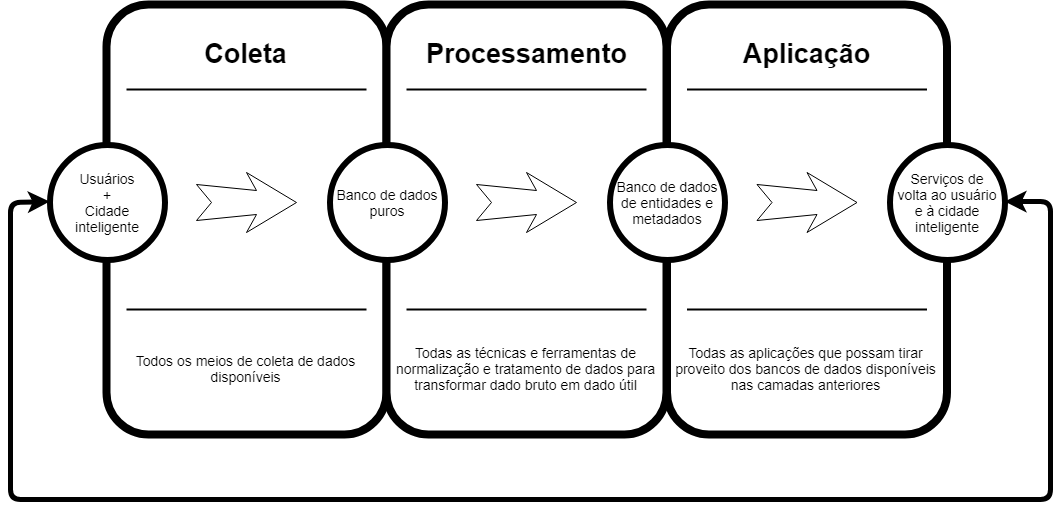
\includegraphics[width=0.8\textwidth]{images/PoorFlow.png}
\end{figure}

\begin{figure}[h]
\caption{abordagem multidimensional}
\centering
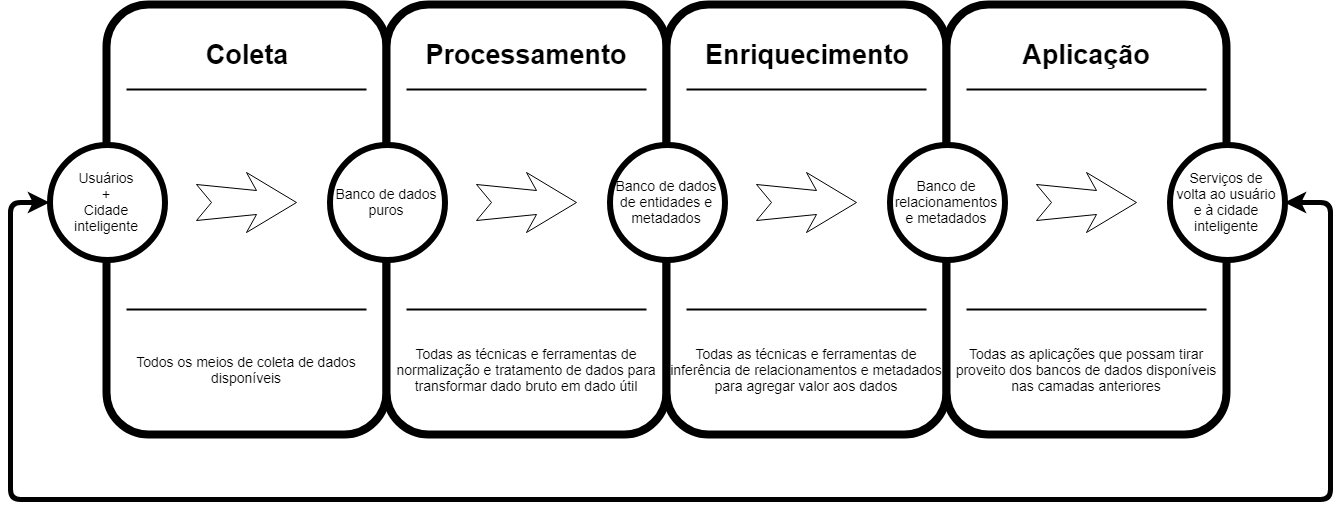
\includegraphics[width=0.8\textwidth]{images/FullFlow.png}
\end{figure}

\section{Estrutura das representações de contexto}

Apesar dos detalhes das etapas do fluxo terem sido descritas anteriormente, a camada de aplicação pode ser considerada agnóstica quanto à implementação dos bancos de dados de entidades, metadados e relacionamentos. Com isso, podemos considerar que a estrutura da representação de contexto de cada um dos cenários confia nas camadas anteriores de maneira transparente.

\newpage

\begin{minted}[
    frame=lines,
    framesep=2mm,
    baselinestretch=0.8,
    fontsize=\footnotesize,
    linenos
]{groovy}
/**
* Defines a single relationship between a document/event and an entity.
* Contains as much metadata as available in the original event
*/
class SD_EntityEventRelationship {
    //mandatory, identifies the data content that generated this relationship
    Event originalEvent
    //mandatory, points to a definition of an entity on an Ontology/Thesaurus
    Entity entity

    //timestamp is so common that we can consider the SD model to have it,
    //but it isn't properly used in the query process
    //optional, with as much precision as possible
    Timestamp timestamp
}

/**
* Defines the query used in a context
* to search for all possible entityEventRelationships,
* in the single-dimension scenario,
* and without considering an oerall multilayered context.
* Note that this match only cares for the {entity} relation:
* it's unaware of time or place, or any other metadata
*/
class SD_ContextQuery {
    Entity entity
}

/**
* Defines the answer to a SD_ContextQuery
*/
class SD_ContextualMatch {
    //this contains all occurencies of the matched entity
    List<EntityEventRelationship> matchHistory

    /**
    * calculated from the distance between the query entity
    * and the matched EntityEventRelationship
    */
    BigDecimal relevance
}
\end{minted}

Blablabla blablabla

\newpage


\begin{minted}[
    frame=lines,
    framesep=2mm,
    baselinestretch=0.8,
    fontsize=\footnotesize,
    linenos
]{groovy}
/**
* Augments the original EntityEventRelationship with all the other
* metadata layers
*/
class MD_EntityEventRelationship extends SD_EntityEventRelationship {
    
    //now mandatory, most of the time with a millisecond precision
    Timestamp timestamp
    //now mandatory, with as much precision as possible
    Coodinates coordinates
    //optional, freeform metadata that doesn't fit time or place concepts
    HashMap extraMetadata

    /**
    * Instead of having simple and single entityEventRelationships,
    * we can provide the API with a way to inspect all neighbours
    * of the one that triggered the match, which will paint
    * the picture of the whole rich original context
    * of all the channels collecting data
    */
    public List<MD_EntityEventRelationship> nearbyEntityEventRelationships() {
        /*...*/
    }
}

/**
* Represents a cluster of EntityEventRelationship that are
* near each other in at least one dimension/attribute.
*
* We can represent this as a cloud of events that have a high
* temporal/georeferencial/semantic relationship between them
*/
class MD_CompositeContextSurface {
    HashMap<MD_EntityEventRelationship, Point> surface
}

/**
* The same as SD_ContextQuery,
* but taking into account all available metadata
*/
class MD_ContextQuery {
    Entity entity

    Timestamp timestamp
    Coodinates coordinates
    HashMap extraMetadata
}

class MD_ContextualMatch {
    //this contains all occurencies of the matched query on all layers and dimensions
    List<MD_CompositeContextSurface> matchHistory

    /**
    * calculated from the collective distance between all attributes
    * of the query and the MD_CompositeContextSurface
    * 
    * a list of distances of each attribute could also be implemented,
    * to supply queries targeted on a single domain, like time
    */
    BigDecimal relevance
}
\end{minted}

Blablabla blablabla

\newpage

\chapter{Desafios} \label{c:desafios}

Dada a larga escala de impacto do sistema proposto por este trabalho, seria impossível esperar que nenhum desafio estivesse entre a situação atual da internet e das ferramentas disponíveis e o estágio desejado e vislumbrado pelos projetos de grandes cidades inteligentes. Na verdade, são vários os desafios em cada uma das camadas de implementação sugeridas, sejam eles técnicos, financeiros , sociais, ou culturais.

\section{Privacidade}

Assim como introduzido na seção \ref{ss:privacidade_na_internet_das_coisas}, considerando a imensa dependência da solução proposta e de projetos de cidades inteligentes de uma excelente e abrangente camada de coleta de dados, privacidade há de ser um dos maiores desafios socioculturais impostos à web semântica e internet das coisas \cite{Kirrane2018PrivacySA}.

Seria impossível atingir excelência de coleta de dados se, por exemplo, todos os canais de dados expostos na seção \ref{s:fontes_de_dados_consideradas} fossem considerados violações de direitos universais de privacidade e propriedade de informação, e portanto proibidos ou banidos de sistemas de cidades inteligentes.

Espera-se que um processo de conscientização, esclarecimento e regulamentação detalhado aconteça nos próximos anos \cite{security:web3.0} - assim como o que teve início com o GDPR (\textit{General Data Protection Regulation}) na Europa - a fim de permitir que a população tenha total ciência dos riscos \textbf{e benefícios} da disponibilização de acesso de dados privados a serviços de terceiros.

\section{Escalabilidade}

Sistemas de recomendação de conteúdo clássicos fazem parte de um privilegiado grupo de técnicas utilizadas neste trabalho que não sofre de problemas de escalabilidade, pois possuem um escopo de \textbf{coleta, armazenamento e processamento} de dados bem definido e limitado.

A inclusão do conceito de metadados - aqui incluindo as dimensões temporais e geoespaciais - eleva a escala destas três etapas ao mundo de sistemas distribuídos multiagentes de processamento em tempo real. Daí, considerar a análise multidimensional para a definição de contexto e para o enriquecimento deste já alcança um patamar de volume de dados para processamento interessante, onde as ferramentas atuais se veem desafiadas. 

Por último, a inclusão deste projeto num cenário de cidades inteligentes ultrapassa as barreiras de volume, variedade e velocidade de dados processáveis com tranquilidade em múltiplas ordens de grandeza\footnote{\href{https://www.zdnet.com/article/volume-velocity-and-variety-understanding-the-three-vs-of-big-data/}{ZDNet: Understanding the three V's of big data}}.

A maior conclusão no tópico de escalabilidade e factibilidade técnica é a de que será necessário um nível de multidisciplinaridade altíssimo, além do uso sincronizado de múltiplas ferramentas especialistas, sempre num modelo de sistemas altamente distribuídos e não-concorrentes.

Qualquer outra tentativa de procura ou utilização de uma ferramenta que resolva todos os problemas com excelência pode colocar o processo de tomada de decisão de sistemas conectados em perigo\footnote{\url{https://www.forbes.com/sites/brentdykes/2017/06/28/big-data-forget-volume-and-variety-focus-on-velocity}}.

\section{Efeitos do mundo digital na evolução humana}

A teoria da seleção natural e processos evolutivos tem sido colocada em cheque na era digital, onde diversas habilidades do ser humano que o diferenciou competitivamente ao longo de centenas de milhares de anos estão se perdendo pela crescente dependência do homem para com as máquinas e sistemas digitais de informação.

Ferramentas de assistência cognitiva, como o motor de busca Google, possuem a maior parcela nessa influência\footnote{\url{https://neurocritic.blogspot.com/2011/07/google-stroop-effect.html}} quando o problema é observado com foco nas últimas duas décadas \cite{Sparrow2011GoogleEO}. 

Vários livros foram escritos sobre a influência da tecnologia sobre os processos biológicos, psicológicos e especialmente cognitivos \cite{theshallows, theglasscage}. Não existe unanimidade: alguns autores detalham uma visão negativa da relação do homem com o processo evolutivo\footnote{\url{http://www.ucl.ac.uk/media/library/humanevolution}}; outros descrevem de maneira otimista como o ser humano tem tomado as rédias do processo evolutivo e está decidindo seu próprio destino evolutivo\footnote{\url{http://www.kurzweilai.net/evolution-and-the-internet-toward-a-networked-humanity}}\footnote{\href{https://www.nationalgeographic.com/magazine/2017/04/evolution-genetics-medicine-brain-technology-cyborg/}{National Geographic: How Humans Are Shaping Our Own Evolution}}.
\chapter{Possibilidades e trabalhos futuros} \label{c:possibilidades_trabalhos_futuros}

Tendo descrito as peças necessárias para compor um sistema completo de coleta, processamento, enriquecimento e aplicação de dados no cenário de cidades inteligentes, podemos mencionar algumas iniciativas e projetos que chamam a atenção pelo potencial de amadurecer o sistema aqui proposto de maneira relevante, e talvez até de atacar e resolver vários dos desafios apresentados ao decorrer do projeto.

\section{SOLID Pods}

Tim Berners-Lee, o pesquisador que arquitetou em 1989, enquanto pesquisador do CERN, a primeira versão do que hoje chamamos de \textbf{Web} (a parte mais visível da internet), vem descrevendo modelos da web semântica há mais de 20 anos, com os primeiros rascunhos, discussões online, e livros \cite{berners2001weaving} datando de 1998\footnote{\url{https://www.w3.org/DesignIssues/Semantic.html}}.

A partir do seu trabalho de pesquisa pelo MIT, sendo membro fundador do World Wide Web Consortium (W3C), Tim vem desenvolvido o modelo de um novo conjunto de ferramentas e abordagens que definitivamente se encaixam em parte do que a suposta Web 3.0 tem como premissa. Em novembro de 2015 o Computer Science and Artificial Intelligence Lab (CSAIL) do MIT publicou\footnote{\href{https://www.csail.mit.edu/news/web-inventor-tim-berners-lees-next-project-platform-gives-users-control-their-data}{CSAIL, MIT, News - Web inventor Tim Berners-Lee's next project}} que o projeto SOLID havia ganho um presente de 1 milhão de dólares da MasterCard como incentivo de pesquisa para o projeto e para o Grupo de Informação Descentralizada (Decentralized Information Group, DIG\footnote{\url{http://dig.csail.mit.edu/}}).

Segue a definição do projeto pelo site do mesmo, em tradução livre do inglês:

\begin{quote}
    Solid (derived from "social linked data") is a proposed set of conventions and tools for building decentralized social applications based on Linked Data principles. Solid is modular and extensible and it relies as much as possible on existing W3C standards and protocols.
\end{quote}

\begin{quote}
    Solid (derivado de "dados sociais interligados") é um conjunto de convenções e ferramentas proposto para construir aplicações sociais descentralizadas baseadas nos princípios de Dados Interligados. Solid é modular e extensível, e se baseia o máximo possível em padrões e protocolos existentes da W3C.
\end{quote}e

O projeto SOLID foi anunciado desde 2016 várias vezes\footnote{\url{https://www.digitaltrends.com/web/ways-to-decentralize-the-web/}}\footnote{\url{https://www.wired.com/2017/04/tim-berners-lee-inventor-web-plots-radical-overhaul-creation/}} pela mídia como uma possível "solução para a web"\footnote{\href{https://www.extremetech.com/extreme/281334-tim-berners-lees-solid-project-can-it-save-the-web}{ExtremeTech - Tim Bernes-Lee's Solid Project: Can it save the web?}}.

Dentre as origens e influências do projeto, estão um projeto de armazenamento social nas nuvens\footnote{\url{https://www.w3.org/DesignIssues/CloudStorage.html}} e um modelo de dados relacionados de escrita e leitura\footnote{\url{https://www.w3.org/DesignIssues/ReadWriteLinkedData.html}}, ambos pela W3C. A primeira obra de pesquisa sobre o projeto é de 2016, com coautoria do próprio Tim Berners-Lee \cite{mansour2016demonstration}. Alguns trabalhos derivados já existem, fazendo uso da plataforma e projeto SOLID para definição de um modelo de notificações com dados interconectados \cite{capadisli2017linked}.

Uma explicação sobre o modo de funcionamento e convenções da ferramenta pode ser encontrado no portal da Inrupt\footnote{\url{https://solid.inrupt.com/how-it-works}}, companhia do próprio Tim Berners-Lee que oferece serviços na plataforma.

\section{Sidewalk Labs}

Filha do conjunto de empresas que compõem a Alphabet Inc. (assim como a Google Inc.), a empresa norte americada Sidewalk Labs é, por definição, uma \textbf{organização de inovação urbana}. Seu objetivo é reimaginar cidades para melhorar a qualidade de vida de seus moradores\footnote{\url{https://www.sidewalklabs.com/}}. Sendo uma das empresas irmãs da Google, e sabendo que esta é uma das maiores presenças no mundo de coleta, processamento, enriquecimento e aplicação de dados no universo da web semântica, a Sidewalk Labs e seus projetos de cidades inteligentes nativamente conectadas têm o potencial de amadurecer vários modelos intermediários ou completos de um sistema como o proposto por este trabalho. Seu projeto principal e inicial é o de revitalização da área de Quayside em Toronto\footnote{\url{https://sidewalktoronto.ca/}}, no Canadá, já nos moldes que definem uma cidade inteligente.

Saber que os projetos da Sidewalk Labs, e futuramente outros projetos de cidades inteligentes derivados, estão nascendo com acesso a todo o conhecimento, \textit{expertise} e tecnologia disponível e amadurecido pela Google, dá uma credibilidade enorme à capacidade desses projetos de alcançarem níveis de arquitetura e eficiência de implementação das etapas descritas neste trabalho.
\chapter{Conclusões} \label{c:conclusao}

O detalhamento das etapas necessárias para a implementação de um sistema de \textbf{coleta, processamento, enriquecimento e aplicação} de dados \textbf{num cenário de cidades inteligentes}, assim como a disposição dos desafios e possíveis problemas que a área de conhecimento denominada por \textbf{análise semântica}, reforça alguns pontos importantes e premissas de uma implementação de sucesso de sistemas como este:

\begin{itemize}
    \item Multidisciplinaridade: o envolvimento de diversas áreas do conhecimento, como neurociência, psicologia, engenharia social, administração, política, desenvolvimento de sistemas computacionais, automação residencial e industrial, dentre diversas outras áreas, é crucial para o bom andamento de um projeto que tem uma área de impacto tão abrangente como este.
    \item Multidimensionalidade: a análise de diversas dimensões dos dados, como as de tempo, localização e de valor semântico, é fundamental para atingir um nível de enriquecimento de contexto eficiente em descrever os diversos cenários da vida real com riqueza e precisão, e então ser capaz de inferir e fazer uso dos relacionamentos mais implícitos e detalhados possíveis.
    \item Governança algorítmica: um modelo completo e detalhado de gestão de acesso às diversas camadas de dados de uma cidade inteligente é uma premissa certa de um projeto de cidade inteligente de sucesso. Sem esse planejamento e execução cuidadoso, os problemas sociais que podem surgir possuem o poder de inviabilizar socialmente todas as etapas previstas por este trabalho.
    \item Privacidade: o aprofundamento no estudo, conscientização e regulamentação do que tange à privacidade do usuário final e cidadão de uma cidade inteligente precisa acontecer com urgência, e iniciativas como o GDPR não podem ser consideradas como burocracia desnecessária, mas sim como parte inerente ao projeto de elevação da web e das cidades a um patamar mais inteligente, e portanto, mais humano.
\end{itemize}

% ----------------------------------------------------------
% Finaliza a parte no bookmark do PDF
% para que se inicie o bookmark na raiz
% e adiciona espaço de parte no Sumário
% ----------------------------------------------------------
%\phantompart


% ----------------------------------------------------------
% ELEMENTOS PÓS-TEXTUAIS
% ----------------------------------------------------------
\postextual
% ----------------------------------------------------------

% ----------------------------------------------------------
% Referências bibliográficas
% ----------------------------------------------------------
\bibliography{references}

% ----------------------------------------------------------
% Glossário
% ----------------------------------------------------------
%
% Consulte o manual da classe abntex2 para orientações sobre o glossário.
%
%\glossary


%---------------------------------------------------------------------
% INDICE REMISSIVO
%---------------------------------------------------------------------
%\phantompart
\printindex
%---------------------------------------------------------------------

\end{document}
